% Copyright 2004 by Till Tantau <tantau@users.sourceforge.net>.
%
% In principle, this file can be redistributed and/or modified under
% the terms of the GNU Public License, version 2.
%
% However, this file is supposed to be a template to be modified
% for your own needs. For this reason, if you use this file as a
% template and not specifically distribute it as part of a another
% package/program, I grant the extra permission to freely copy and
% modify this file as you see fit and even to delete this copyright
% notice. 

\documentclass{beamer}
\usepackage[utf8]{inputenc}
\usepackage[brazilian]{babel}
\usepackage{color}

% There are many different themes available for Beamer. A comprehensive
% list with examples is given here:
% http://deic.uab.es/~iblanes/beamer_gallery/index_by_theme.html
% You can uncomment the themes below if you would like to use a different
% one:
%\usetheme{AnnArbor}
%\usetheme{Antibes}
%\usetheme{Bergen}
%\usetheme{Berkeley}
%\usetheme{Berlin}
%\usetheme{Boadilla}
%\usetheme{boxes}
\usetheme{CambridgeUS}
%\usetheme{Copenhagen}
%\usetheme{Darmstadt}
%\usetheme{default}
%\usetheme{Frankfurt}
%\usetheme{Goettingen}
%\usetheme{Hannover}
%\usetheme{Ilmenau}
%\usetheme{JuanLesPins}
%\usetheme{Luebeck}
%\usetheme{Madrid}
%\usetheme{Malmoe}
%\usetheme{Marburg}
%\usetheme{Montpellier}
%\usetheme{PaloAlto}
%\usetheme{Pittsburgh}
%\usetheme{Rochester}
%\usetheme{Singapore}
%\usetheme{Szeged}
%\usetheme{Warsaw}

\title{Aula Introdutória - Unix}

% A subtitle is optional and this may be deleted
\subtitle{Curso de Unix}

\author{PET Computa\c{c}ão}
% - Give the names in the same order as the appear in the paper.
% - Use the \inst{?} command only if the authors have different
%   affiliation.

\institute[UFSC] % (optional, but mostly needed)
{
%
  Departamento de Informática e Estatística\\
  Universidade de Santa Catarina}
% - Use the \inst command only if there are several affiliations.
% - Keep it simple, no one is interested in your street address.

\date{PET Computa\c{c}ão, 2015}
% - Either use conference name or its abbreviation.
% - Not really informative to the audience, more for people (including
%   yourself) who are reading the slides online

\subject{Curso de Unix}
% This is only inserted into the PDF information catalog. Can be left
% out. 

% If you have a file called "university-logo-filename.xxx", where xxx
% is a graphic format that can be processed by latex or pdflatex,
% resp., then you can add a logo as follows:

% \pgfdeclareimage[height=0.5cm]{university-logo}{university-logo-filename}
% \logo{\pgfuseimage{university-logo}}

% Delete this, if you do not want the table of contents to pop up at
% the beginning of each subsection:
\AtBeginSubsection[]
{
  \begin{frame}<beamer>{Sumário}
    \tableofcontents[currentsection,currentsubsection]
  \end{frame}
}

% Let's get started
\begin{document}

\begin{frame}
  \titlepage
\end{frame}

\begin{frame}{Sumário}
  \tableofcontents
  % You might wish to add the option [pausesections]
\end{frame}

% Section and subsections will appear in the presentation overview
% and table of contents.
\section{Por que utilizar Linux?}

\subsection{Imagens comuns no Windows}

\begin{frame}{Por que utilizar Linux?}{Imagens comuns no windows}
    \begin{figure}[h!]
        \centering
        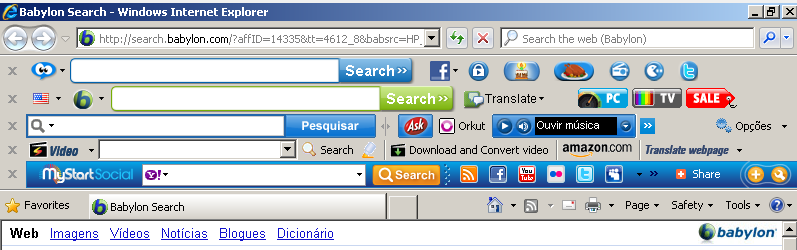
\includegraphics[scale=0.40]{toolbars.png}
    \end{figure}
\end{frame}

\begin{frame}{Por que utilizar Linux?}{Imagens comuns no windows}
    \begin{figure}[h!]
        \centering
        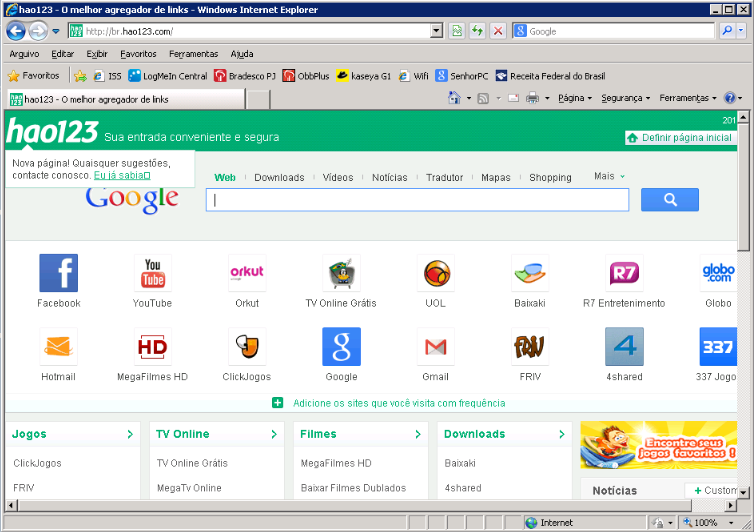
\includegraphics[scale=0.3]{hao123.png}
    \end{figure}
\end{frame}

\begin{frame}{Por que utilizar Linux?}{Imagens comuns no windows}
    \begin{figure}[h!]
        \centering
        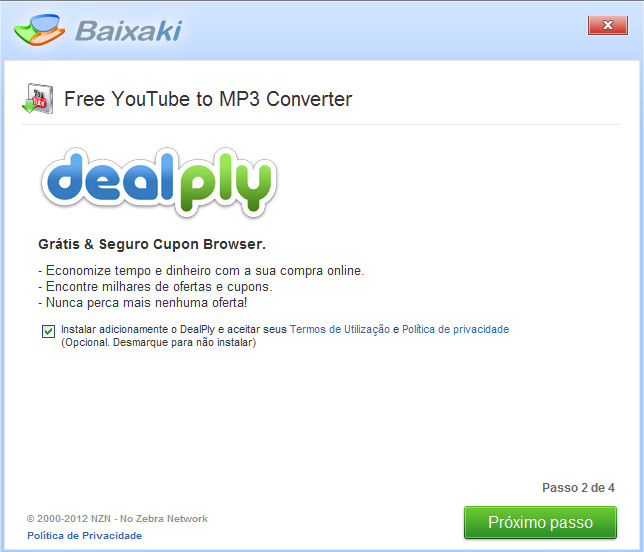
\includegraphics[scale=0.3]{dealply.jpg}
    \end{figure}
\end{frame}

\subsection{"Degradação" do Windows vs "Degradação do Linux}
\begin{frame}{"Degradação" do Windows}{Após formatado}
    \begin{figure}[h!]
        \centering
        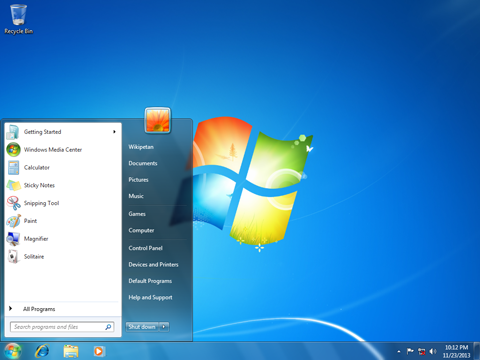
\includegraphics[scale=0.5]{Windows_7.png}
    \end{figure}
\end{frame}

\begin{frame}{"Degradação" do Windows}{Após um mês de uso}
    \begin{figure}[h!]
        \centering
        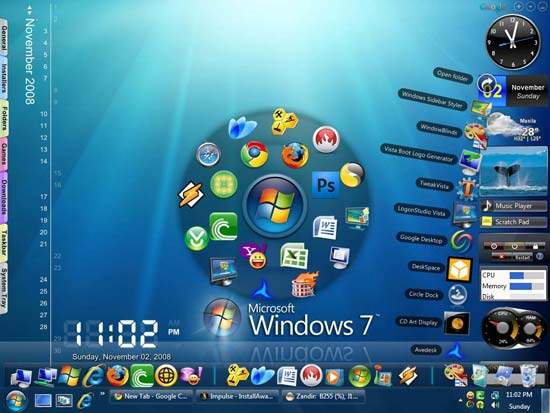
\includegraphics[scale=0.4]{ruindows7.jpg}
    \end{figure}
\end{frame}

\begin{frame}{"Degradação" do Linux}{Após formatado}
    \begin{figure}[h!]
        \centering
        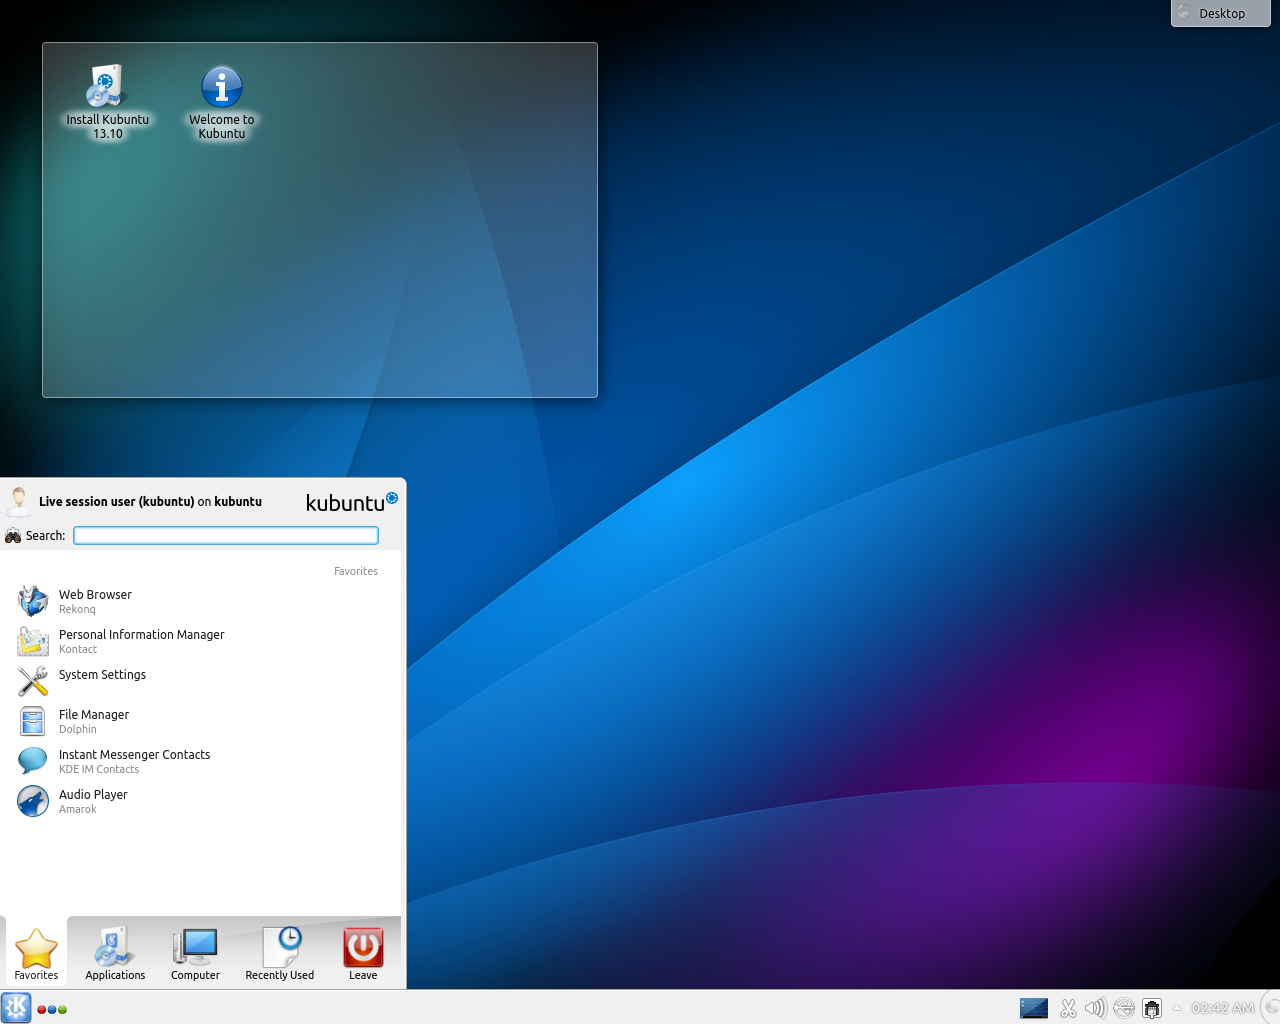
\includegraphics[scale=0.25]{Kubuntu.png}
    \end{figure}
\end{frame}


\begin{frame}{"Degradação" do Linux}{Após um mês de uso}
    \begin{figure}[h!]
        \centering
        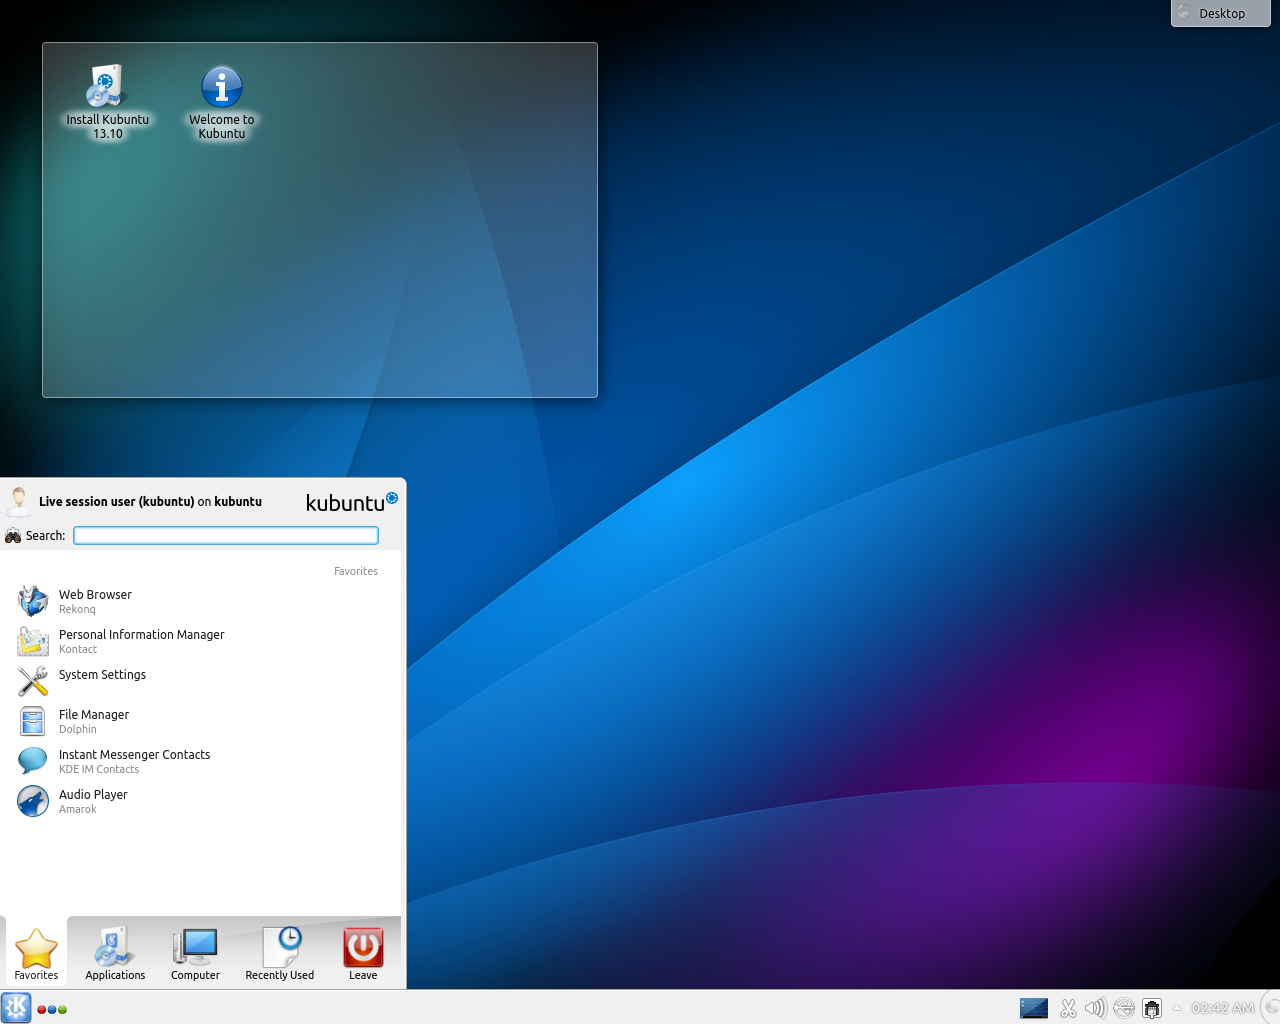
\includegraphics[scale=0.25]{Kubuntu.png}
    \end{figure}
\end{frame}

\subsection{Valor de instalação}
\begin{frame}{Valor da instalação}
    \begin{itemize}
        \item{Você pode baixar e instalar seu linux direto das páginas na web dos desenvolvedores sem custo algum.}
\item{Quando você compra o seu computador que já vem com Windows, você paga o valor da licença no preço final do computador, e muito provavelmente terá que formatá-lo após algum tempo de uso e gastará mais dinheiro na formatação.}
    \end{itemize}
\end{frame}


\subsection{Suporte livre na internet vs Suporte pago on-line}
\begin{frame} 
\begin{itemize}
        \item{Quando algum problema acontece no seu linux, você encontra várias pessoas na internet que tiveram o mesmo erro, conseguiram corrigir e colocaram a correção lá para você não passar o mesmo trabalho que eles.}
\item{No Windows, quando você se depara com algum problema, você tem duas opções: Ligar para um técnico ou contactar o suporte on-line do Windows (caso seu Windows não for pirateado).}
    \end{itemize}
\end{frame}

\subsection{Considerações Finais}
\begin{frame} 
\begin{figure}[h!]
        \centering
        
\includegraphics[scale=0.3]{Tux.png}
    \end{figure}
\begin{itemize}
\item{Após estes pontos levantados, deixarei pra você tirar suas conclusões.}
    \end{itemize}
\end{frame}

\end{document}


